\documentclass[a4paper]{article}

\usepackage[utf8]{inputenc}
\usepackage[T1]{fontenc}
\usepackage{textcomp}
\usepackage{mathtools,amssymb,amsthm}
\usepackage[top=2.5cm,bottom=2.5cm,right=2.5cm,left=2.5cm]{geometry}
\usepackage[francais]{babel}

%============header and foot============
\usepackage{fancyhdr}
\pagestyle{fancy}
\renewcommand\headrulewidth{1pt}
\fancyhead[L]{CHASSAGNOL Rémi}
\fancyhead[R]{2020-2021}

%================infos=================
\title{Réalité virtuelle et imagerie}
\author{CHASSAGNOL Rémi}
\date{\today}

%================image=================
\usepackage{graphicx}
\graphicspath{{figures/}}


\begin{document}
  \maketitle  

  \section{Organisation des classes}%
  \label{sec:Organisation des classes}

  Une expression binaire est un arbre qui contient la décomposition de
  l'expression, où chaque nœud contient une sous expression et chaque feuille
  contient une variable ou une constante. Pour modéliser cet arbre à l'aide de
  Java, on utilisera une classe \textbf{Expression} qui représentera
  l'expression et contiendra la racine de l'arbre de l'expression. L'arbre sera
  composé de \textbf{node} qui est une interface qui sera implémentée par des
  classes représentants des littéraux (variables ou constantes) ou des
  opérations (addition, soustraction, multiplication, division). Voici le
  diagramme UML des classes ci-dessous:

  \begin{figure}[h]
    \centering
  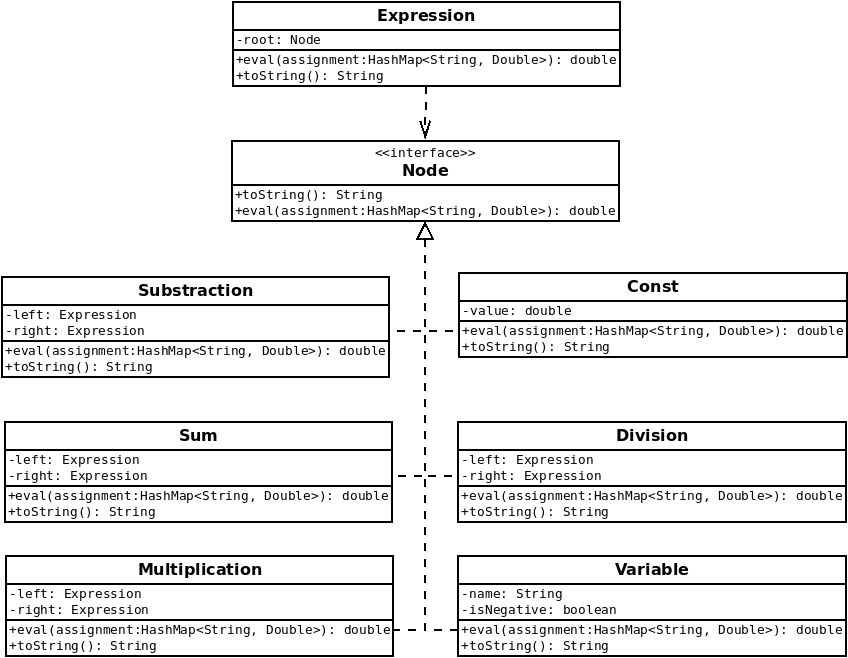
\includegraphics[scale=0.5]{./Diagram_uml.png}
    \caption{Diagramme des classes}%
    \label{fig:Diagramme des classes}
  \end{figure}

  \subsection{Expression}%
  \label{sub:Expression}

  La classe \textbf{Expression} possède un attribut privé \textbf{root} qui est
  la racine de l'arbre. Cette classe possède deux constructeurs, le premier
  permet de générer une expression depuis un nœud, et le second permet de
  générer une expression depuis une chaîne de caractères contenant une
  expression binaire écrite en utilisant la convention \textbf{préfixe} (ex:
  \texttt{(+ 2 2)}). Enfin, la classe possède deux méthodes publiques,
  \textbf{toString} qui permet d'afficher la formule (avec la convention
  infixe: \texttt{(2 + 2)}) et \textbf{eval} qui prend pour paramètre une
  \texttt{HashMap<String, double>} contenant les couples \textbf{[nomVariable :
  valeurVariable]} (les valeurs affectées aux variables de la formules) et qui
  retourne le résultat de la formule sous forme de \texttt{double}.

  A noter que cette classe possède aussi des méthodes privées utilisées pour
  extraire une expression des expressions de la chaîne de caractères donnée en
  paramètre au second constructeur.

  \subsection{L'interface nœud}%
  \label{sub:L'interface noeud}

  Chaque nœud de l'arbre doit posséder deux méthodes: \textbf{eval} et
  \textbf{toString} permettant l'évaluation et l'affichage de la formule.
  Cependant, bien que nous les nœuds possèdent ces méthodes, les expressions
  binaires (addition, \dots), les variables et les constantes ne possèdent pas
  les mêmes attributs ni les mêmes implémentations de ces méthodes, il est donc
  logique de préférer l'utilisation d'une interface à l'utilisation d'une classe
  abstraite. De ce fait, une \textbf{Expression} peut manipuler une addition et
  une variable de la même façon.

  \subsection{Les implémentations de nœud}%
  \label{sub:Les implémentations de noeud}

  \subsubsection{Variables et constantes}%
  \label{ssub:Variables et constantes}

  La classe \textbf{variable}  possède deux attributs privés, \textbf{name} qui
  contient le nom de la variable et \textbf{isNegative} qui est un booléen qui
  contient \texttt{vrai} si la variable est négative dans la formule (ce qui
  n'a rien à voir avec sa valeur, une variable \textbf{var} peut contenir les
  valeurs 5 ou -12 mais être utilisé en tant que \textbf{-var} dans la
  formule). La méthode \textbf{eval} retourne la valeur correspondant à
  \textbf{name} dans la \texttt{HashMap} \textbf{assignment} (et la modifie en
  fonction de \textbf{isNegative}). La méthode \textbf{toString} retourne
  \texttt{name} ou \texttt{"-" + name} en fonction de \texttt{isNegative}.

  La classe \textbf{constante} possède un attribut privé double qui contient sa
  valeur et implémente les méthodes \textbf{eval} qui retourne la valeur et
  \textbf{toString} qui retourne la valeur sous la forme d'une chaîne de
  caractères.

  \subsubsection{Expressions binaires}%
  \label{ssub:Expressions binaires}

  Les quatre expressions binaires sont très similaires, elles possèdent toutes
  deux attributs privés \textbf{left} et \textbf{right} qui contiennent les
  sous expressions de gauche et de droite de l'expression (ex: \texttt{left +
  right}). La seule différence se trouve dans les méthodes \textbf{eval} et
  \textbf{toString}, \textbf{eval} va effectuer l'addition de \textbf{left} et
  \textbf{right} dans le cas de \textbf{Sum}, la soustraction dans le cas de
  \textbf{Substraction}, \dots et \textbf{toString} va retourner \texttt{"left
  c right"} en remplaçant \textbf{c} par le caractère correspondant à
  l'opération.
  
  \section{Récupération d'une formule}%
  \label{sec:Récupération d'une formule}
  
  \subsection{Le constructeur de Expression}%
  \label{sub:Le constructeur de Expression}
  
  Pour rappel, la classe \textbf{Expression} possède deux constructeurs, le
  premier génère une expression binaire à partir de deux sous-expressions et
  le second prend en paramètre une chaîne de caractères qui contient une
  expression mathématique écrite selon la convention préfixe (de plus, on
  suppose que l'expression donnée est une expression binaire et non pas une
  constante ou une variable). Avant de commencer l'extraction de l'expression,
  on commence par remplacer tous les potentiels "bloques d'espaces" (plusieurs
  espaces à la suite) et tabulation par un espace simple, ce qui rend
  l'utilisation des indices dans la chaîne possible (par exemple, on devient
  sûr que le quatrième caractère de la chaîne est soit le début d'une opération
  binaire \textbf{'('}, soit le premier caractère d'un littéral) et permet de
  corriger de potentielles erreurs de l'utilisateur. Ensuite, on distingue
  quatre cas qui correspondent à quatre formes possibles de
  l'expression:

  \begin{itemize}
    \item \textbf{cas 1: (. x y)}, opération entre deux littéraux x et y,
    \item \textbf{cas 2: (. (...) x)}, opération entre une sous opération binaire suivie d'un littéral x,
    \item \textbf{cas 3: (. x (...))}, une opération entre un littéral x suivi d'une sous opération binaire,
    \item \textbf{cas 4: (. (...) (...))}, une opération entre deux sous-opérations binaires. 
  \end{itemize}
  
  De ce fait, on sait exactement ce que l'on a à extraire, et donc quelle
  méthode appeler pour construire les parties gauche et droite de l'expression.

  \subsection{Les méthodes d'extractions}%
  \label{sub:Les méthodes d'extractions}

  Ces méthodes servent uniquement au second constructeur de la classe
  \textbf{Expression} et ne doivent pas pouvoir être appelées par l'utilisateur
  de l'objet, elle sont donc définies comme étant privées pour respecter
  l'encapsulation de l'objet Expression.

  \subsubsection{Récupération d'une expression depuis une String}%
  \label{ssub:Récupération d'une expression depuis une String}

  Cette méthode est une procédure qui va modifier (par effet de bord) le
  tableau \textbf{expressionParts} (qui doit contenir les partie gauche
  \texttt{[0]} et droite \texttt{[1]} de l'expression). Si une des parties de
  l'expression est un littéral, la case de \textbf{expressionParts}
  correspondant contiendra une chaîne de caractères vide à la fin de
  l'exécution ce qui permet de traiter les quatre cas vus précédemment dans le
  second constructeur de \textbf{Expression}.
  
  Cette méthode se divise en deux parties, dans un premier temps, on récupère
  une première opération binaire en se servant de la variable
  \textbf{formulaLevel} pour compter les parenthèses (pour récupérer la bonne
  chaîne si il y a des parenthèses dans les parenthèses) et d'une boucle
  \textbf{do while}. A noter qu'à la fin de cette première partie, la première
  case de \textbf{expressionParts} contient la première opération binaire
  trouvée dans la chaîne, si la première partie de l'expression est un littéral
  (et la seconde, une opération binaire), on vient de récupérer la seconde
  partie.

  Ensuite, on teste si il reste une opération binaire à extraire (on regarde
  l'indice de la prochaine \textbf{'('} et si c'est -1, c'est qu'il n'y en a
  pas), si c'est le cas, on récupère la fin de la chaîne dans
  \textbf{expressionParts[1]} et on se retrouve dans le \textbf{cas 4}. Dans le
  cas contraire, on regarde si le quatrième caractère est une \textbf{'('} (i.e.
  que la première partie de l'expression est une opération binaire), si c'est
  le cas, on ne fait rien et on se retrouve dans le \textbf{cas 2}, sinon, on
  échange les valeurs dans les cases de \textbf{expressionParts} pour se
  retrouver dans le \textbf{cas 3}.
  
  \subsubsection{Extraction d'un littéral}%
  \label{ssub:Extraction d'un littéral}

  Cette méthode est appelée dans le \textbf{cas 1} et elle permet de récupérer
  les deux littéraux gauche et droit de l'expression.

  \subsubsection{Création d'un littéral}%
  \label{ssub:Création d'un littéral}

  La méthode \textbf{createExpressionFromLitteral} permet de créer une
  \textbf{Expression} qui est une \textbf{constante} ou une \textbf{variable} à
  partir d'une chaîne de caractères. Cette méthode fait appel à la méthode
  \textbf{isNumeric} qui retourne \textbf{vrai} si la chaîne de caractères
  passée en paramètre contient un double. Pour cela, cette méthode fait un
  \textbf{try} pour tester si la méthode \textbf{Double.parseDouble} lève une
  exception \textbf{NumberFormatException}, si c'est le cas, la chaîne ne
  contient pas un double et donc c'est un nom de variable, sinon, elle contient
  la valeur d'une constante.

  \subsubsection{Création d'une expression}%
  \label{ssub:Création d'une expression}
  
  Une fois que l'on a les parties gauche et droite d'une expression, on peut
  faire appel à la fonction \textbf{createOperation} qui crée un nœud (qui
  sera affecté à l'attribut \textbf{root} de \textbf{Expression}) en
  utilisant les sous-expressions et le signe de l'expression préalablement
  récupéré.
  
  
  
\end{document}
